%% Final Knowledge-Based Systems supplementary source.
\documentclass[a4paper,fleqn]{cas-sc}

\usepackage[numbers,sort&compress]{natbib}
\usepackage{amsmath}
\usepackage{amssymb}
\usepackage{booktabs}
\usepackage{array}
\usepackage{graphicx}
\usepackage{xurl}
\usepackage{amsthm}
\usepackage{multirow}
\usepackage{makecell}
\usepackage{hyperref}
\hypersetup{colorlinks=true,linkcolor=blue,citecolor=blue,urlcolor=blue}

\newtheorem{lemma}{Lemma}

\begin{document}
\let\WriteBookmarks\relax
\def\floatpagepagefraction{1}
\def\textpagefraction{.001}
\pagenumbering{arabic}

\shorttitle{Supplementary Material}
\shortauthors{Ma and Wang}

\title[mode=title]{Supplementary Material for Structurally-Calibrated Functional Attribution: A Methodology for Process Supervision Weighting in Reflective Reasoning}

\author[1]{Haoran Ma}
\ead{mahaoran0000@foamail.com}

\author[1,2]{Ningning Wang\corref{cor1}}
\ead{wangningning@bistu.edu.cn}

\cortext[cor1]{Corresponding author.}

\affiliation[1]{organization={College of Management Science and Engineering, Beijing Information Science and Technology University},
            city={Beijing},
            postcode={102200},
            country={China}}

\affiliation[2]{organization={Institute of Information Systems, ESG Intelligent Application Innovation Research Center},
            city={Beijing},
            postcode={102200},
            country={China}}

\begin{abstract}
This supplementary material provides notation details, proof sketches, additional experimental results, KBS pilot details, and reproducibility notes for the SC-FMA manuscript. It also records the validation boundary: GSM8K/HotpotQA replay and downstream filtering are failed or blocked provenance, while the Countries KG study is a fixture-level pilot over real KG structure.
\end{abstract}

\begin{keywords}
supplementary material \sep structural calibration \sep reproducibility \sep knowledge graph pilot
\end{keywords}

\maketitle

\section{Notation Reference}

Table~\ref{tab:notation} summarizes the notation used in the main text. Vectors are column vectors, $\|\cdot\|_2$ denotes the Euclidean norm, and $\odot$ denotes elementwise multiplication.

\begin{table}[h]
\caption{Notation used by SC-FMA.}
\label{tab:notation}
\centering
\small
\begin{tabular}{lll}
\toprule
\textbf{Symbol} & \textbf{Meaning} & \textbf{Domain} \\
\midrule
$k$ & Number of reflective steps & $k \in \mathbb{N}$ \\
$\tau$ & Reasoning trace & Text sequence with identified spans \\
$\mathcal{G}$ & Reflection DAG & $(\mathcal{V},\mathcal{E})$ \\
$c_i$ & Local CIU for step $i$ & Protocol-dependent utility difference \\
$n_i$ & Structural necessity for step $i$ & $[0,1]$ \\
$R_{ij}$ & Redundancy between steps $i,j$ & $[0,1]$ after PSD correction \\
$b_i$ & Bottleneck indicator & $\{0,1\}$ \\
$w_i$ & Calibrated supervision weight & $w_i \ge \varepsilon$ \\
$\alpha,\beta,\gamma,\delta$ & SCU trade-off weights & Nonnegative hyperparameters \\
\bottomrule
\end{tabular}
\end{table}

\section{Optimization Details}

The SCU objective is:
\begin{equation}
L(\mathbf{w}) =
\alpha\|\mathbf{w}-\tilde{\mathbf{c}}\|_2^2
+\beta\|\mathbf{w}-\tilde{\mathbf{n}}\|_2^2
+\gamma\mathbf{w}^{\top}\mathbf{R}\mathbf{w}
-\delta\sum_i b_i\log(w_i),
\end{equation}
with $\mathbf{w}$ constrained to the simplex $\mathcal{W}=\{\mathbf{w}: w_i\ge \varepsilon,\sum_i w_i=1\}$.

\subsection{KKT conditions}

For the constrained optimum $\mathbf{w}^{*}$, the Karush--Kuhn--Tucker conditions are:
\begin{align}
\frac{\partial L}{\partial w_i}\bigg|_{\mathbf{w}^{*}}-\mu_i^{*}-\lambda^{*}&=0, \\
\mu_i^{*}&\ge 0, \\
\mu_i^{*}(w_i^{*}-\varepsilon)&=0, \\
w_i^{*}&\ge \varepsilon, \\
\sum_i w_i^{*}&=1.
\end{align}
The derivative is:
\begin{equation}
\frac{\partial L}{\partial w_i} =
2\alpha(w_i-\tilde{c}_i)+2\beta(w_i-\tilde{n}_i)+2\gamma(\mathbf{R}\mathbf{w})_i-\delta b_i/w_i.
\end{equation}

\subsection{Variance-reduction intuition}

If $\gamma=\delta=0$, the unconstrained minimizer is:
\begin{equation}
\hat{\mathbf{w}}=\frac{\alpha\tilde{\mathbf{c}}+\beta\tilde{\mathbf{n}}}{\alpha+\beta}.
\end{equation}
The calibrated vector therefore shrinks raw CIU toward structural necessity. Projection onto the simplex is non-expansive~\cite{wang2013projection}, so the constrained solution cannot amplify deviations in the same way direct raw-CIU weighting can. The main text reports the empirical consequence: SC-FMA QP improves ranking correlation over raw CIU while reducing sensitivity to noisy local utility.

\section{Additional Experimental Results}

\subsection{Per-size ranking results}

\begin{table}[h]
\caption{Step importance ranking metrics stratified by trace size $k$. Values are mean Spearman $\rho$.}
\label{tab:per-size}
\centering
\small
\begin{tabular}{lccccc}
\toprule
\textbf{Method} & $k=3$ & $k=4$ & $k=5$ & $k=6$ & $k \ge 7$ \\
\midrule
SC-FMA QP & 0.582 & 0.601 & 0.615 & 0.622 & 0.634 \\
SC-FMA Ridge & 0.521 & 0.534 & 0.540 & 0.538 & 0.542 \\
SC-FMA Projection & 0.328 & 0.341 & 0.345 & 0.339 & 0.342 \\
Raw CIU & 0.471 & 0.485 & 0.490 & 0.482 & 0.486 \\
\bottomrule
\end{tabular}
\end{table}

The improvement of SC-FMA QP over raw CIU grows with trace size, consistent with the mechanism that redundancy and bottleneck structure become more informative in larger reflection DAGs.

\subsection{Structural diagnostic figures}

\begin{figure}[h]
\centering
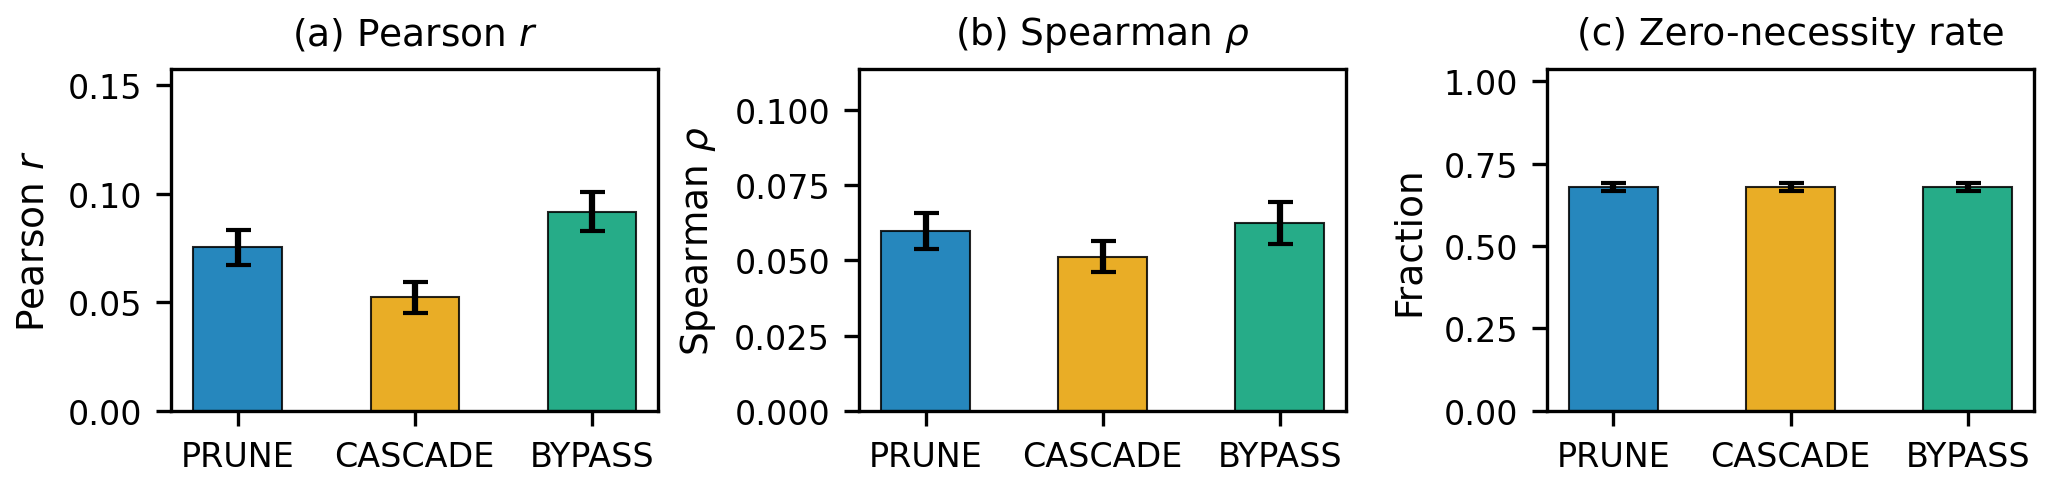
\includegraphics[width=0.85\linewidth]{figures/fig_mode_comparison.png}
\caption{Structural diagnostic summary by perturbation mode. PRUNE, CASCADE, and BYPASS produce consistently weak CIU-necessity alignment.}
\label{fig:mode-comparison}
\end{figure}

\begin{figure}[h]
\centering
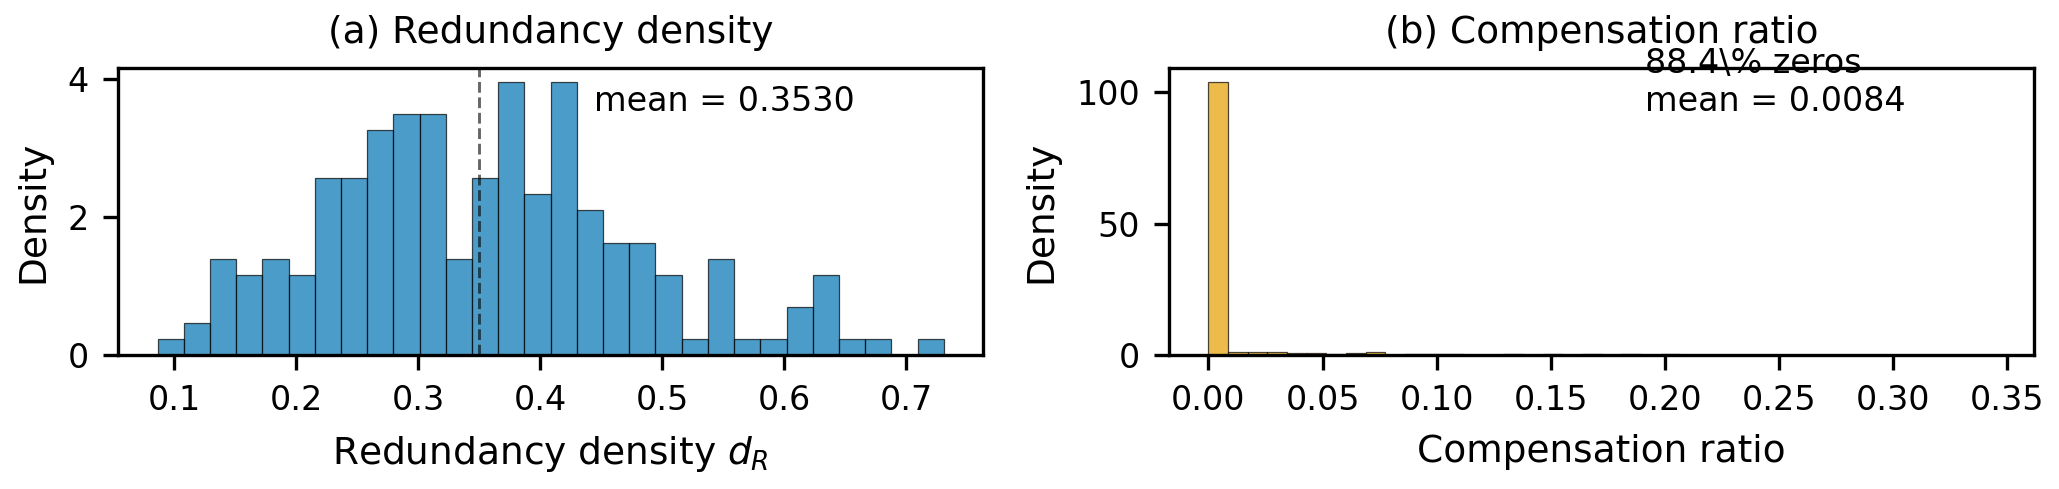
\includegraphics[width=0.85\linewidth]{figures/fig_redundancy_comp.png}
\caption{Redundancy and compensation diagnostics. Compensation is concentrated near zero, showing that removing a node rarely increases downstream necessity enough to replace it.}
\label{fig:redundancy}
\end{figure}

\begin{figure}[h]
\centering

\includegraphics[width=0.85\linewidth]{figures/fig_resilience.png}
\caption{Resilience curves under ordered node removal. Necessity-first removal degrades structural support faster than attribution-first or random removal.}
\label{fig:resilience}
\end{figure}

\clearpage

\section{KBS Pilot Details}

The Countries KG pilot is a small deterministic pilot over real KG structure~\cite{bordes2013translating}. It uses 25 country entities, 5 region entities, and 189 triples. The graph layer adds ontology-derived edges from \texttt{locatedIn} and \texttt{neighborOf} relations, then compares structural diagnostics with the baseline TF-IDF reflection DAG. The pilot result records \texttt{validated\_kbs\_workflow=false}: it checks ontology-aware edge construction feasibility, not deployed KBS correctness.

\begin{table}[h]
\caption{KBS evidence boundary.}
\label{tab:kbs-boundary}
\centering
\small
\begin{tabular}{lll}
\toprule
\textbf{Evidence item} & \textbf{Status} & \textbf{Claim supported} \\
\midrule
Synthetic SC-FMA benchmark & Completed & Controlled calibration mechanism \\
PRM800K locked labels & Completed with overlap limits & Real step-label ranking context \\
Countries KG pilot & Pilot & Ontology-aware edge construction feasibility \\
GSM8K/HotpotQA replay & Failed/blocked & Provenance only \\
Downstream filtering & Failed/blocked & No performance-improvement claim \\
Rule-engine deployment & Not evaluated & Future work only \\
\bottomrule
\end{tabular}
\end{table}

\section{Reproducibility Notes}

All reported synthetic experiments use deterministic seeds, fixed graph-construction parameters, and frozen hyperparameters after validation-set tuning. The source package includes both the manuscript and supplementary LaTeX sources, bibliography, CAS style files, and all figures used in the submission. Build artifacts are intentionally excluded from the upload source zip.

\section{Submission Statements}

\section*{Funding}
This work was supported by the National Social Science Fund of China Project (24BSH018) and the Beijing Natural Science Foundation Project (L252145).

\section*{Declaration of Competing Interest}
The authors declared that they have no conflicts of interest to this work.

\section*{Data Availability}
Data will be made available on request.

\bibliographystyle{cas-model2-names}
\bibliography{references}

\end{document}
